\section{Introduction}
%We employ a search and prune in the graph of state space to learn action classifiers for each query class. At test time given the current state (previous detector responses and the current image) representing by the CNN features of the masked search space, the action classifier will select the most highly scored action. We also incorporate early rejection as an action which will reject further detection if the it isn't likely to contain the query object in the current masks. 

Object detection and segmentation in complex scenes is a central and challenging problem in computer vision and robotics.
%Given an image, for example, Figure~\ref{fig:20Qintro}, our goal is to answer the query: is there a car in the scene, and if yes, to locate it with a bounding box or pixel-wise labels.
This problem is usually tackled by running multiple object detectors exhaustively on densely sampled sliding windows~\cite{felzenszwalb2010object} or category-independent object proposals~\cite{carreira2012cpmc,van2011segmentation,arbelaez2014multiscale}. 
Such methods are time-consuming since they need to evaluate a large number of object hypotheses, and can easily introduce false positives if exclusively considering local appearance.
% In addition, due to variations in data distribution, occlusion and viewpoint change, object models may not always capture the appearance of objects and ambiguity arises. 
%In the example of Figure~\ref{fig:20Qintro}, since the viewpoint and the scale of the cars are not similar to those in common training images, it is difficult for the car detector to recognize and locate them.

Instead of checking all hypotheses indiscriminately and exhaustively, humans only look for a set of related objects in a given context~\cite{biederman1982scene, hock1974contextual}. Context information is an effective cue for humans to detect low-resolution or small objects in cluttered scenes~\cite{parikh2012exploring}. Many contextual models have been proposed to capture relationships between objects at the semantic level to reduce ambiguities from
unreliable independent detection results~\cite{gould2009decomposing, ladicky2010graph}. %For example, because roads and buildings often co-occur with cars, knowing the existence of these objects can help us infer the locations of cars.  
However, such methods still need to evaluate the high order co-occurrence statistics and spatial relations of the query object with \emph{all} other object classes in the scene, some of which may not be informative and even introduce unnecessary confusion.  

By contrast, humans do not process the whole scene at once: human visual perception is an active process that sequentially samples the optic array in an intelligent, task-specific way~\cite{najemnik2005optimal}. Research in neuro-science has revealed that when humans search for a target, those objects that are associated to the query will reinforce attention with the query and weaken recognition of unrelated distractions~\cite{moores2003associative}. 
%This is highly inefficient since many non-informative contextual objects have to be queried. 
For instance, in Figure~\ref{fig:20Qintro}, when we search for cars, knowing the top of the scene is sky does not help distinguish whether the image contains either a car or a boat since both are equally likely to be under the sky; 
on the other hand, observing a road instead of water in the lower part gives a strong indication of the existence of cars. 
Therefore, in order to find cars, humans tend to first look for roads instead of sky; additionally, if we can not find cars on the road,  we may want to look ``beside'' the buildings because cars are likely to park next to them. %And if we know there is road, we do not need to ask about water.
%We note that the set of related object classes and the order of asking questions about them is dynamic given a specific query in the scene and knowledge of previous observations.
This motivates us to raise the question: \textit{can object detection algorithms decide where to look for objects of a query class more efficiently and accurately by exploring a few related context cues dynamically, similar to humans?}

We formulate this object detection problem as a Markov Decision Process (MDP). 
We use imitation learning to learn a context-driven policy that sequentially and dynamically selects the most informative context class to explore based on past observations, and gradually refine the search area for the query class. 
We show our framework in Figure~\ref{fig:flowchart}.  Specifically, like playing a Twenty Questions game, at each step the policy asks for information about a context class based on the query and responses from previous contextual classifiers. 
We then run the detector/classifier of the selected context class. Based on the responses, we further refine the search area for the query class using spatially-aware contextual models. 
This process of contextual querying and search area refinement is repeated until the policy determines that sufficient contextual information has been gathered and decides to stop. 
Finally, we run the query object detector in the refined search area and output the result. 
Besides asking for contextual information, our policy can reject a query early to avoid unnecessary detection if it determines that there is little chance of the query object in the scene. 
The early rejection decision can be taken even before running the object detector; therefore we can eliminate a large amount of unnecessary computation. 

Object detection experiments on the PASCAL VOC dataset show that our algorithm produces a search area that has better overlap with the target object by leveraging its context, 
thus significantly reducing the number of object proposals to consider and detectors to evaluate by over $30\%$.
Even with less computation, our method achieves mean average precision (mAP) comparable to or even higher than the exhaustive search method. 
To the best of our knowledge, this is one of the first approaches that solves the challenging task of simultaneous object detection and segmentation in complex scenes in an MDP framework by applying imitation learning to learn a policy fully driven by context.


\begin{figure*}[!tb]
\begin{center}
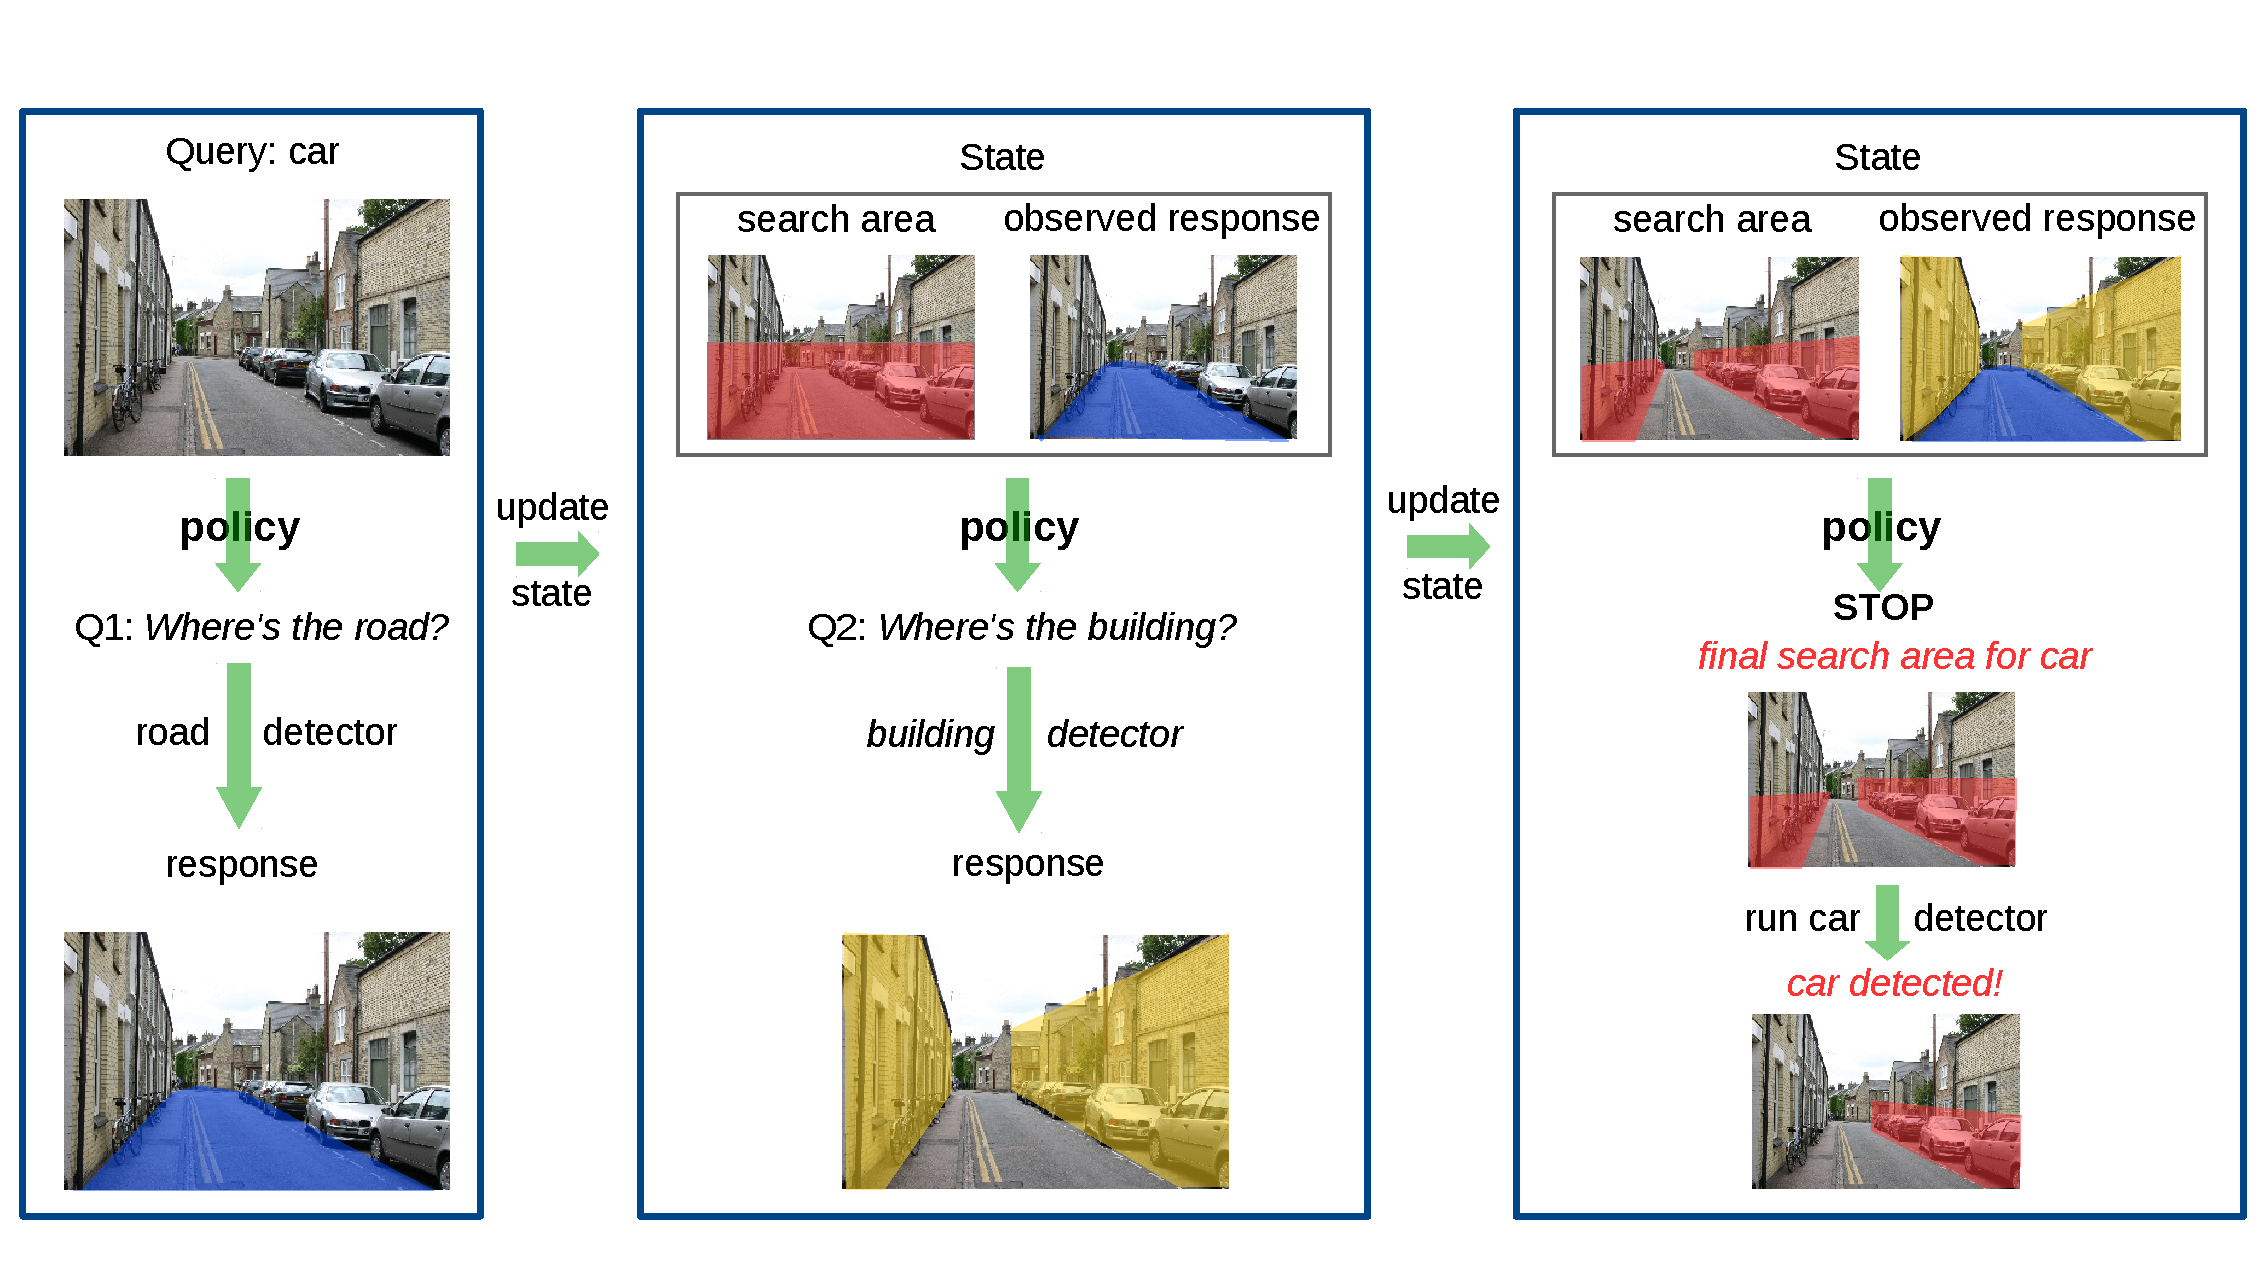
\includegraphics[width=\linewidth]{figures/iccv20q-overview.pdf}
\vspace{-1em}
\caption{Illustration of our sequential search for query objects in 20 context-driven questions.}
\label{fig:20Qintro}
\end{center}\vspace{-2em}
\end{figure*}

% The main contributions of the paper are:
% \HHNote{seems contribution 1 and 2 can be combined, they are both novelty of a new learning algorithm to the problem. e.g., we formulate and learn...}
% \begin{itemize}
% \item a novel formulation of the object detection problem as a Markov Decision Process and a dynamic, closed-loop policy learned by imitation learning to decide which detectors to run next and where to look for the query object iteratively
% \item a general and unified probabilistic framework incorporating responses from multi-class object detectors and contextual classifiers to update the search area for the target
% \item a data-driven context model that not only encodes co-occurrence but also spatial relations by efficient weighted vote maps from exemplars\HHNote{This is not explained before and it's hard to understand here what the context model is}.
% \end{itemize}




